\section{Relazioni}
\begin{definition}[Relazione]
Prendiamo in considerazione un prodotto cartesiano con due insieme A, B che sia A X B = $\{(a,b) \: | \: a \in A, b \in B\} = $ U (Universo). 
\\Una relazione è $R \subseteq U$ dove, come scritto sopra, U = A X B. In una relazione A è detto \textbf{insieme di partenza} e B è detto \textbf{insieme di arrivo}.
\end{definition}
\hspace{-15pt}In sintesi possiamo definire una relazione come un sottoinsieme del prodotto cartesiano fra due insiemi.\\
L'insieme $rel(A,B)$ è l'inseme di tutte le possibili relazioni fra A e B.
\begin{example}
    Esempio relazione.\\\\
    Prendiamo due insiemi e facciamo il prodotto cartesiano.\\
    $S = \{$luca, mario, angela, gino, maria$\}$. Insieme degli studenti.\\
    $C = \{$PA, LAB, FI, AN$\}$. Insieme dei corsi.\\ \\
    Il prodotto cartesiano fra S e C è uguale a tutte le possibile coppie ordinate che si possono formare fra i due insieme, quindi: \hspace{.2cm}
    S X C = $\{$(luca, PA), (luca, LAB), ..., (marica, AN)$\}$.\\ \\
    In questo caso possiamo creare una relazione del prodotto cartesiano andando appunto a prendere un sottoinsieme di A X B andando a stabilire una regola o condizione per scegliere quali coppie ordinate vogliamo nella nostra relazione, esempio:\\
    $R \subseteq$ A X B è una relazione che specifica quali esami sono stati sostenuti dai vari studenti.
\end{example}
\subsection{Identità}
L'identità è un altro tipo di operazione che è possibile fare sulle relazioni, oltre a quelle insiemistiche.
\begin{definition}[Identità]
Preso un insieme A, l'identità su A è una relazione con se stessa, e si scrive $Id_A \subseteq$ A X A, quindi si può vedere come nell'identità di un insieme ogni elementi è identico a se stesso. Inoltre l'identità di un insieme si definisce come:
\end{definition}
\vspace{-20pt}
\begin{equation}
    Id_A = \{(a,a) \: | \: a \in A\}
\end{equation}
\vspace{-20pt}
\subsection{Composizione}
\begin{definition}[Composizione]
La composizione, date due relazioni $R \subseteq$ A X B e $S \subseteq$ B X C si scrive R;S e sarebbe una relazione che si sviluppa fra gli elementi degli insiemi diversi di R ed S, in questo caso A e C, che però hanno uno stesso collegamento ad un elemento dell'insieme B. Matematicamente si definisce come:
\end{definition}

\begin{equation}
    R;S = \{(a, c) \in A \: X \: C \: \: | \: \: \exists \: b \in B \: \: . \: \: (a,b) \in R  \land (b,c) \in S\}
\end{equation}
\\
\textbf{NOTA:} l'insieme di arrivo di R deve essere uguale all'insieme di partenza di S per effettuare l'operazione di composizione.
\\
\begin{wrapfigure}{l}{8cm}
    \vspace{-15pt}
    \centering
    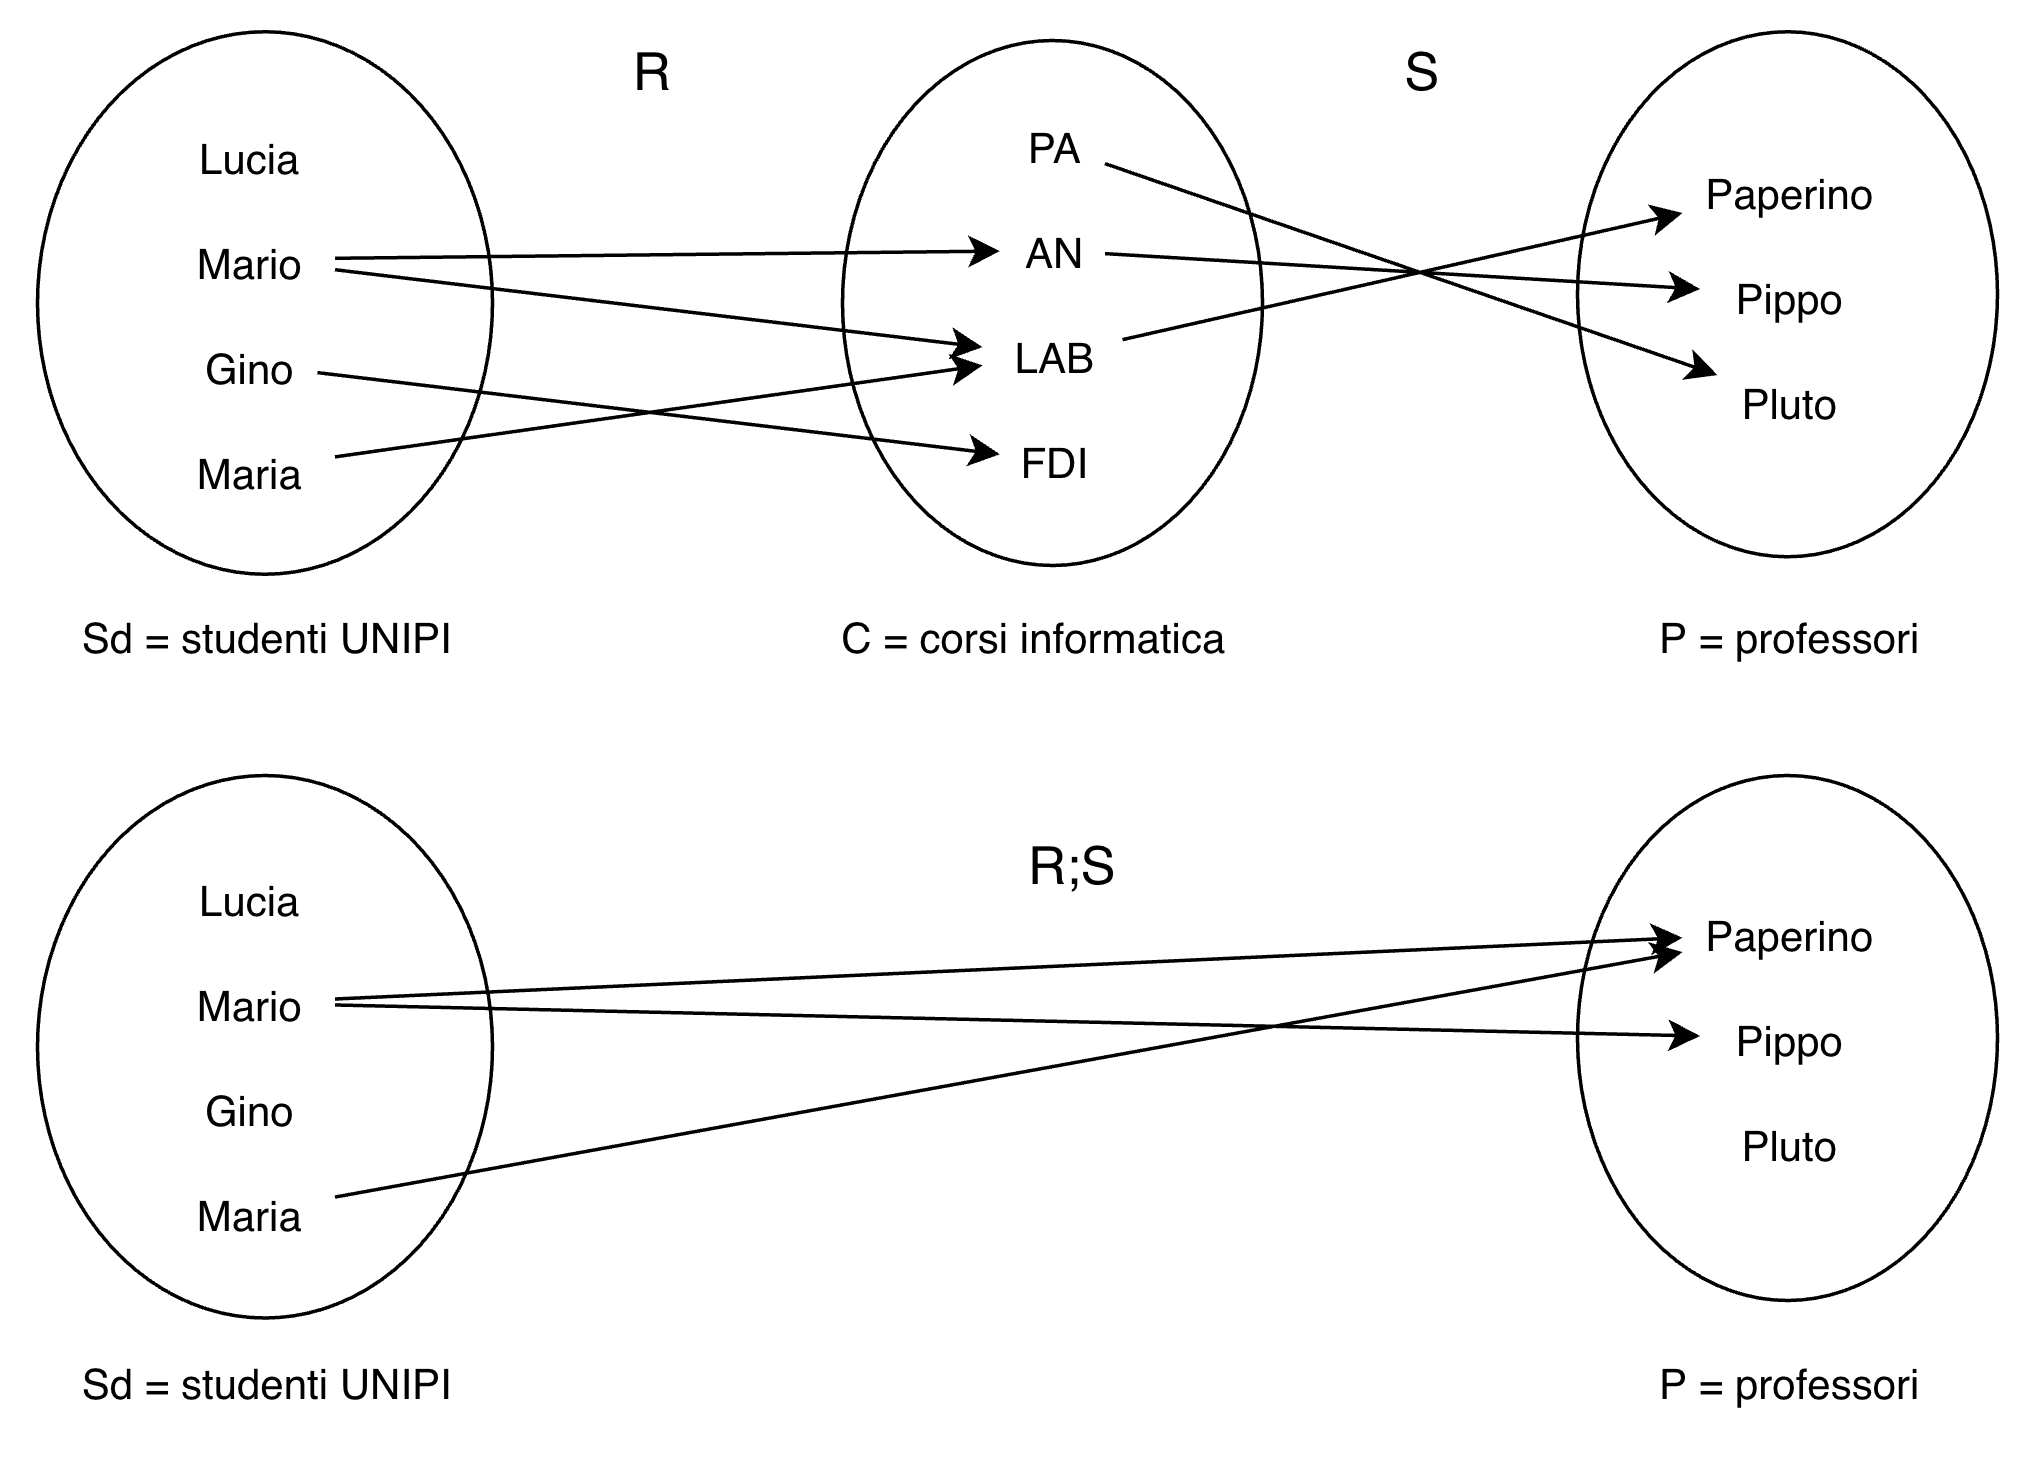
\includegraphics[width=7.2cm]{esempio-composizione.png}
    \caption{Esempio composizione}
    \label{fig:esempio-composizione}
\end{wrapfigure}
\begin{example}
\vspace{-15pt}
Nell'esempio in figura [\ref{fig:esempio-composizione}] prendiamo in considerazione i seguenti insiemi:\\ \\
$Sd = \{$lucia, mario, gino, maria$\}$\\
$C = \{$PA, LAB, FI, AN$\}$\\
$P = \{$paperino, pippi, pluto$\}$ \\ \\
Effettuiamo un'operazione di composizione. Come possiamo vedere il risultato è un insieme che unisce gli elementi di Sd e P che avevano una relazione con un elemento di C in comune.\\
\end{example}

\subsection{Relazione opposta}
\begin{definition}[Relazione opposta]
Dato un insieme A e B ed una relazione $R \subseteq$ A X B, una relazione opposta è inversione dell'associazione degli elementi degli insiemi A e B da (a,b) a (b,a) e si definisce formalmente come: $R^{op} = \{(b, a) \in$ B X A $|$ $(a,b) \in R\}$
\end{definition}

\begin{example}
    A = $\{$pagine web$\}$ \hspace{.5cm} B = $\{$parole del vocabolario$\}$ \hspace{.5cm} $R \subseteq$ A X B\\
    Si associa ciascuna pagina web con le parole in essa contenuta:
    \begin{itemize}
        \item $(a,b) \in \mathbb{R}$ dice che nella pagina web "a" è contenuta la parola "b".
        \item $R^{op}$ ($(b,a) \in \mathbb{R}$) dice per ogni parola "b" quali sono le pagine web che le contengono.
    \end{itemize}
\end{example}

\subsection{Leggi}
Come per gli insiemi, anche per le relazioni esistono delle utili leggi che regolano il comportamento delle varie operazioni. Le relazioni, essendo di base degli insieme, valgono le stesse leggi scritte nella sezione degli insiemi, tabella \ref{tab:leggi-insiemi}. \\ \\
Per tutti gli insiemi A, B, C, D e per tutte le relazioni $R \subseteq A \: X \: B$, $S \subseteq B \: X \: C$, $T \subseteq C \: X \: D$, valgono le leggi scritte nelle tabelle \ref{tab:leggi-composizione}, \ref{tab:leggi-relazioni-opposte}, \ref{tab:leggi-distributività}.
\begin{table}[h!]
    \setlength{\tabcolsep}{8pt}
    \renewcommand{\arraystretch}{2}
    \centering
    \begin{tabular}{|c|c|}
    \hline
        \textbf{Associatività} & (R;S);T = R;(S;T) \\ 
        \textbf{Unità} & $Id_A$;R = R;$Id_B$ = R \\
        \textbf{Assorbimento} & $\O$;S = S;$\O$ = $\O$ \\ \hline
    \end{tabular}
    \caption{Leggi composizione}
    \label{tab:leggi-composizione}
\end{table}
\begin{table}[h!]
    \vspace{-10pt}
    \centering
    \setlength{\tabcolsep}{8pt}
    \renewcommand{\arraystretch}{2}
    \begin{tabular}{|c|c|}
        \hline
        \textbf{Convoluzione} & $(R^{op})^{op} = R$ \\
        \textbf{Opposto-identità} & $(Id)^{op} = Id$ \\
        \textbf{Opposto-complemento} & $($A X B$)^{op}$ = (B X A) \\
        \textbf{Opposto-vuoto} & $(\O)^{op} = \O$ \\ \hline
    \end{tabular}
    \caption{Leggi relazioni opposte}
    \label{tab:leggi-relazioni-opposte}
\end{table}
\begin{table}[h!]
    \vspace{-10pt}
    \centering
    \setlength{\tabcolsep}{8pt}
    \renewcommand{\arraystretch}{2}
    \begin{tabular}{|c|c|c|}
        \hline
        \textbf{Distributività composizione} & R;(S $\cup$ T) = (R;S) $\cup$ (R;T) & (S $\cup$ T); R = (S;R) $\cup$ (T;R) \\
        \textbf{Distributività opposto} & $(R \cup S)^{op}$ = $S^{op} \cup R^{op}$ & $(R \cap S)^{op}$ = $S^{op} \cap R^{op}$ \\
        \textbf{Distributività opposto su negazione} & $(\overline{R})^{op} = (\overline{R^{op}})$ & \\
        \textbf{Distributività opposto su composizione} & $($R;S$)^{op}$ = $S^{op}$;$R^{op}$ & \\ \hline
    \end{tabular}
    \caption{Leggi distributività}
    \label{tab:leggi-distributività}
\end{table}
\\
\textbf{Spiegazione Associatività:}\\
R;S $\subseteq$ A X C, facendo la composizione con T la prima parte dell'uguaglianza (R;S);T $\subseteq$ A X D. A sua volta, analizzando la seconda parte dell'uguaglianza, S;T $\subseteq$ B X D che poi se andiamo a comporre con R risulta che R;(S;T) $\subseteq$ A X D. Possiamo così vedere che l'uguaglianza è verificata. Per la dimostrazione discorsiva completa vedere in seguito. \\ \\
\textbf{Spiegazione Unità:}\\
Essendo che $Id_A$ = A X A e $Id_B$ = B X B vediamo che la prima parte dell'uguaglianza $Id_A$;R = A X B e la seconda è R;$Id_B$ = A X B, quindi la prima uguaglianza è verificata. La seconda uguaglianza si verifica in automatico visto che A X B è uguale a R.


\subsubsection{Dimostrazione proprietà associativa}
\begin{demostration}
    Facciamo una dimostrazione discorsiva della proprietà associativa in tabella \ref{tab:leggi-composizione}.\\
    Proprietà associativa: (R;S);T = R;(S;T) \hspace{.3cm} Con: $R \subseteq$ A X B, \: \: $S \subseteq$ B X C, \: \: $T \subseteq$ C X D.\\ \\
    \textit{Innanzitutto ricordiamo la proprietà per cui dati 2 insiemi X, Y $X = Y \Longleftrightarrow X \subseteq Y \land Y \subseteq X$.} \\
    Utilizziamo la proprietà sopra scritto andando a sostituire alla X "(R;S);T" e alla Y "R;(S;T)", troviamo così due condizioni che, per l'operatore logico $\land$, devono essere vere entrambe per far valere l'uguaglianza:
    \begin{itemize}
        \item (R;S);T $\subseteq$ R;(S;T) - \underline{Dimostrazione 1°}.
        \item R;(S;T) $\subseteq$ (R;S);T - \underline{Dimostrazione 2°}.
    \end{itemize}
        \underline{Dimostrazione 1°}: (R;S);T $\subseteq$ R;(S;T) \\ 
        \textit{Come prima cosa ricordiamo che un insieme $W \subseteq Z \: \: \forall \: w \in W \land z \in Z$.} \\
        Sostituendo "(R;S);T" a W e "R;(S;T)" a Z troviamo che, per fare in modo che la condizione che un insieme sia sottoinsieme di un altro $\forall \: (a,d) \in$ (R;S);T $ \land \: (a,d) \in$ R;(S;T). \footnote{Ricordati che (R;S);T ha al suo interno coppie (a,d) $\subseteq$ A X D per le operazioni di composizione}\\ \\
        Noi dobbiamo dimostrare che $\forall \: (a,d) \in$ R;(S;T) sia vera:\\
        Prendiamo come prima cosa una generica coppia di valori (a,d) $\in$ (R;S);T. Perché esista questa coppia deve esistere per forza un valore "c" che faccia da ponte fra "(R;S)" e "T" (ricordiamo che R;S $\subseteq$ A X C e T $\subseteq$ C X D). Possiamo scrivere quindi (Colore \textbf{nero} nella rappresentazione [\ref{fig:rappresentazioni-dim-associtiva}]):
        \begin{equation}
            (a,d) \in (R;S);T \Longrightarrow \: \exists \: c \in C \: \bullet (a,c) \in R;S \land (c,d) \in T \text{ (Nel disegno freccia NERA)}
            \label{eq:dim1-associtiva-1}
        \end{equation}
        Ora nella forma scritta sopra [\ref{eq:dim1-associtiva-1}] abbiamo una parte (a,c) $\in$ R;S che deve essere "scomposta" in maniera specifica per verificare che tutta la composizione di partenza sia vera, infatti deve esistere un valore b che colleghi l'insieme R ed S nell'operazione di composizione R;S (ricordiamolo che R $\subseteq$ A X B e R $\subseteq$ B X S). Possiamo scrivere quindi (Colore \textbf{blu} nella rappresentazione [\ref{fig:rappresentazioni-dim-associtiva}]):
        \begin{equation}
            (a,d) \in (R;S);T \Longrightarrow \: \exists \: b \in B, \: c \in C \: \bullet (a,b) \in R \land (b,c) \in S \land (c,d) \in T \text{ (Nel disegno freccia BLU)}
            \label{eq:dim1-associtiva-2}
        \end{equation}
        Ora per arrivare alla forma che dobbiamo dimostrare, R;(S;T), l'ultima forma [\ref{eq:dim1-associtiva-2}] è troppo estesa, infatti la parte $(b,c) \in S \land (c,d) \in T$ deve essere racchiusa per arrivare alla forma S;T. Quindi andiamo a scrivere che (Colore \textbf{rosso} nella rappresentazione [\ref{fig:rappresentazioni-dim-associtiva}]):
        \begin{equation}
            (a,d) \in R;(S;T) \Longrightarrow \: \exists \: b \in B \bullet (a,b) \in R \land (b,d) \in S;T \text{ (Nel disegno freccia ROSSA)}
            \label{eq:dim1-associtiva-3}
        \end{equation}
        L'ultima forma raggiunta [\ref{eq:dim1-associtiva-3}] dimostra che $\forall \: (a,d) \in$ R;(S;T) è vera e quindi che (R;S);T $\subseteq$ R;(S;T) è verificata. $\blacksquare$
        \begin{figure}[h!]
            \centering
            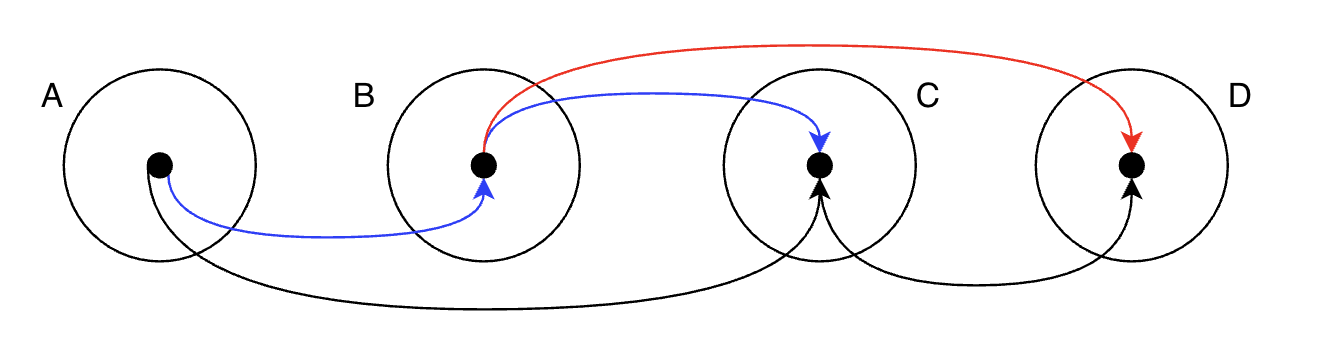
\includegraphics[width=10cm]{dimostrazione-associtiva.png}
            \vspace{-10pt}
            \caption{Rappresentazione dimostrazione 1°}
            \label{fig:rappresentazioni-dim-associtiva}
        \end{figure}
        \\\\
        \underline{Dimostrazione 2°}: R;(S;T) $\subseteq$ (R;S);T\\
        La seconda dimostrazione ha uno svolgimento analoga alla prima. Pure qui andiamo a considerare che: per fare in modo che la prima parte, cioè "R;(S;T)", sia sottoinsieme della seconda, la seconda deve contenere tutti gli elementi della prima. quindi $\forall (a,d) \in R;(S;T) \: \land \:(a,d) \in (R;S);T$. \\ \\Per fare in modo che ciò scritto sia vero dobbiamo dimostrare che $\forall \: (a,d) \in (R;S);T$ sia vero:\\
        Come prima cosa dobbiamo capire in che casi i punti appartengono a "(R;S);T", questo avviene quando esiste un punto "c" che collega "R;S" e "T" (R;S è uguale a A X C e T è C X D), quindi possiamo scrivere che:
        \begin{equation}
            (a,d) \in (R;S);T \Longrightarrow \forall c \in C \: \bullet \: (a,c) \in R;S \land (c,d) \in T
            \label{eq:dim2-associtiva-1}
        \end{equation}
        Da questo punto procediamo come nella dimostrazione 1° quindi andiamo a scomporre ulteriormente la forma [\ref{eq:dim2-associtiva-1}] in $(a,c) \in R;S$ per verificare i casi in cui la composizione esista:
        \begin{equation}
            (a,d) \in (R;S);T \Longrightarrow \: \exists \: b \in B, \: c \in C \: \bullet (a,b) \in R \land (b,c) \in S \land (c,d) \in T
            \label{eq:dim2-associtiva-2}
        \end{equation}
        L'ultimo passaggio è trasformare la forma [\ref{eq:dim2-associtiva-2}] in una versione che possa validare $\forall \: (a,d) \in (R;S);T$, ed essa sarebbe:
        \begin{equation}
            (a,d) \in R;(S;T) \Longrightarrow \: \exists \: c \in C \bullet (a,c) \in R;S \land (c,d) \in T
            \label{eq:dim2-associtiva-3}
        \end{equation}
        L'ultima forma travata [\ref{eq:dim2-associtiva-3}] verifica che $\forall \: (a,d) \in (R;S);T$ sia vero, di conseguenza pure R;(S;T) $\subseteq$ (R;S);T è verificato. $\blacksquare$\\ \\
        Dato che siamo riusciti a dimostrare entrambe le dimostrazioni la proprietà associativa ((R;S);T = R;(S;T)) con cui siamo partiti è verificata. $\blacksquare$
\end{demostration}


\subsection{Proprietà fondamentali}
Prendendo in considerazioni due insiemi A e B ed una relazione R, dove R $\subseteq$ A X B, valgono le seguenti proprietà.\\ \\
\textbf{Totale:} $\forall \: \: a \in A \bullet \exists \: \: b \in B \bullet (a, b) \in R$ \hfill \textbf{Surgettiva:} $\forall \: \: b \in B \bullet \exists \: \: a \in A \bullet (a, b) \in R$
\begin{figure}[h!]
    \vspace{-8pt}
    \begin{subfigure}{.3\textwidth}
        \centering
        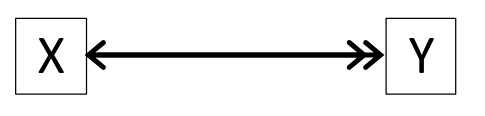
\includegraphics[width=6cm]{totale.png}
        \caption{Ogni elem. di A è collegato ad almeno uno di B}
    \end{subfigure}
    \hspace{4.3cm}
    \begin{subfigure}{.3\textwidth}
        \centering
        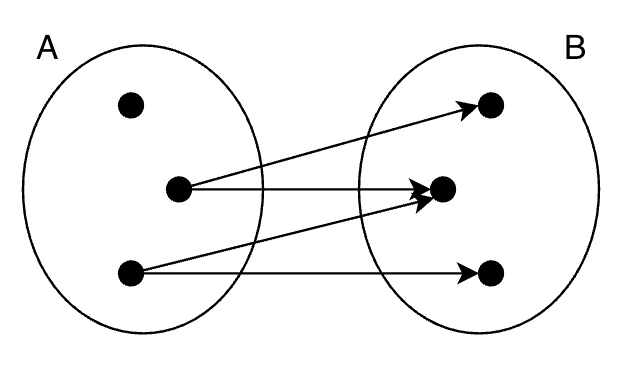
\includegraphics[width=6cm]{surgettiva.png}
        \caption{Ogni elem. di B ha almeno un entrata da A}
    \end{subfigure}
\end{figure}
\\
\textbf{Univalente:} \hspace{6.3cm} \textbf{Iniettiva:}\\ $\forall \: \: a \in A \bullet \exists$ al più un $b \in B \bullet (a, b) \in R$ \hspace{2.4cm}  $\forall \: \: b \in B \bullet \exists$ al più un $a \in A \bullet (a, b) \in R$
\begin{figure}[h!]
    \vspace{-7pt}
    \begin{subfigure}{.3\textwidth}
        \centering
        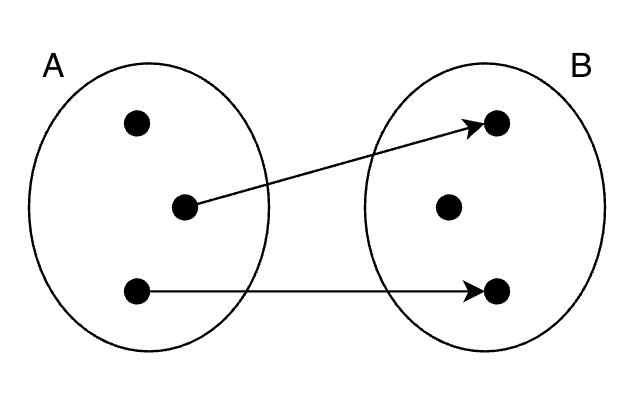
\includegraphics[width=6.2cm]{univalente.png}
        \caption{Ogni elem. di A deve avere al massimo 1 collegamento con B}
    \end{subfigure}
    \hspace{4.3cm}
    \begin{subfigure}{.3\textwidth}
        \centering
        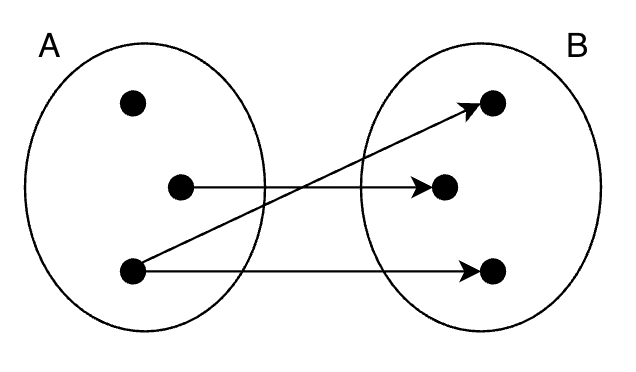
\includegraphics[width=6cm]{iniettiva.png}
        \caption{Ogni elem. di B deve avere al massimo un entrante da A}
    \end{subfigure}
\end{figure}
\\
Le proprietà fra di loro sono legate da un rapporto di dualità in particolare totale con surgettiva e univalente con iniettiva, questo vuol dire che:
\begin{itemize}
    \item R $\subseteq$ A X B è totale $\Longleftrightarrow$ $R^{op} \subseteq$ B X A è surgettiva.
    \item R $\subseteq$ A X B è surgettiva $\Longleftrightarrow$ $R^{op} \subseteq$ B X A è totale.
    \item R $\subseteq$ A X B è univalente $\Longleftrightarrow$ $R^{op} \subseteq$ B X A è iniettiva.
    \item R $\subseteq$ A X B è iniettiva $\Longleftrightarrow$ $R^{op} \subseteq$ B X A è univalente.
\end{itemize}

\subsubsection{Teorema di caratterizzazione}\label{teorema-caratterizzazione}
Prendendo due insiemi A e B ed una relazione R tale che R $\subseteq$ A X B. Possiamo vedere come ogni proprietà fondamentale vale solo se sono soddisfatte delle condizioni che le caratterizzano:
\begin{itemize}
    \item R \textbf{Totale} $\Longleftrightarrow \: Id_A \subseteq R;R^{op}$ - Spiegazione:\\
    La congiunzione fra R che è A X B e il suo opposto che è B X A torna un insieme A X A, per questo l'identità di A ($Id_A$), che sarebbe un insieme A X A, è un sottoinsieme di $R;R^{op}$.\\
    Se R non fosse totale vorrebbe dire che alcuni elementi di R(A) non sono collegati.
    \item R \textbf{Univalente} $\Longleftrightarrow \: R^{op};R \subseteq Id_B$ - Spiegazione:\\
    La congiunzione fra $R^{op}$ che sarebbe B X A e R, che è A X B, forma un insieme B X B che è quindi sottoinsieme di $Id_B$, che sarebbe B X B.
    \item R \textbf{Surgettiva} $\Longleftrightarrow \: Id_B \subseteq \: R^{op};R$ - Spiegazione:\\
    La congiunzione fra $R^{op}$ ed R, che sono rispettivamente B X A e A X B, torna una relazione B X B, quindi $Id_B$, che è B X B, è sottoinsieme.
    \item R \textbf{Iniettiva} $\Longleftrightarrow \: R;R^{op} \subseteq Id_A$ - Spiegazione: \\
    La congiunzione fra R ed $R^{op}$ torna A X A, essendo che R è A X B e l'opposto è B X A, che è sottoinsieme di $Id_A$ che è A X A.
\end{itemize}

\subsubsection{Proprietà di chiusura per composizione}
Per tutti gli insiemi A, B, C e per tutte le relazioni, R $\subseteq$ A X B e S $\subseteq$ B X C valgono le seguenti proprietà:
\begin{enumerate}
    \item Se R ed S sono totali allora la loro composizione R;S è totale.
    \item Se R ed S sono univalenti allora la loro composizione R;S è univalente.
    \item Se R ed S sono surgettive allora la loro composizione R;S è surgettiva.
    \item Se R ed S sono iniettive allora la loro composizione R;S è iniettiva.
\end{enumerate}

\subsection{Funzione}
Una funzione può essere definita utilizzando le proprietà fondamentali delle relazioni.
\begin{definition}[Funzione]
Dati due insiemi A, B ed una relazione R $\subseteq$ A X B, tale relazioni si definisce funzione quando rispetta la proprietà \textbf{totale} e \textbf{univalente} quindi tutti gli elementi dell'insieme A hanno uno ed un solo corrispettivo in B.
\end{definition}
Una funzione è inoltre infittiva quando rispetta la proprietà iniettiva e suriettiva quando rispetta quella surgettiva.
\begin{definition}[Funzione parziale]
    Una funzione si dice parziale se rispetta solamente la proprietà univalente.
\end{definition}
\begin{definition}[Biezione]
Dati due insiemi A, B ed una relazione R $\subseteq$ A X B, tale relazioni si definisce funzione biettiva quando rispetta tutte e 4 le proprietà.
\end{definition}
\begin{example}
    Esempio con i booleani:\\
    bool = $\{$True, False$\}$ \hspace{1cm} 2 = $\{0, 1\}$\\
    Questi due insiemi sono biettivi.
\end{example}
\textbf{Domanda:} Se dati due insiemi A, B dove $|A| \neq |B|$ la loro relazione R $\subseteq$ A X B può essere una biezione?\\
La risposta è NO visto che avendo cardinalità diverse esisterà sempre un elemento in B che o non ha corrispettivo o ne ha 2.

\subsubsection{Composizione fra funzioni}
La composizione fra funzioni è una casistica particolare di quella fra relazioni.
\begin{example}
    Dati due funzioni f e g dove:\\
   $f: A \longrightarrow B$ \hspace{.5cm} $g: B \longrightarrow C$ \footnote{Scrivere una funzione "f" nella forma $f: A \longrightarrow B$  equivale a scrivere f $\subseteq$ A X B}\\ 
    La compozione si scrive come f;g e sarebbe f;g $\subseteq$ A X C \footnote{è possibile scrivere la composizione fra funzioni anche come $g \bullet f$ oppure $g(f())$.}\\ \\
    \textbf{NOTA:} indichiamo con $fun(A,B) = \{f | f: \: A \longrightarrow B\}$ l'insieme di tutte le funzioni che vanno da A a B.
\end{example}

\subsubsection{Proprietà di chiusura per funzioni}
Per tutti gli insiemi A, B, C e per tutte le relazioni, funzioni, $i: A \longrightarrow B$ e $j: B \longrightarrow C$ valgono le seguenti proprietà:
\begin{enumerate}
    \item $Id_A$ è una biezione, essendo che sarebbe una relazione con se stesso.
    \item Se prendiamo $i: A \longrightarrow B$ e $j: B \longrightarrow C$, dove entrambi le funzioni sono biezioni, la loro composizioni, i;j: $A \longrightarrow C$ è a sua volta una biezioni.
    \item Se prendiamo la funzione $i: A \longrightarrow B$ biettiva, il suo opposto $i^{op}: B \longrightarrow A$ è a sua volta biettiva.
\end{enumerate}

\subsubsection{Caratterizzazione in biezione}\label{caratterizzazione-biezione}
\begin{definition}[Caratterizzazione]
In maniera rigorosa la caratterizzazione, applicata alla biezione, si definiscine:
$\forall \: A, B \: \bullet \: \forall \: R \subseteq$ A X B, R è biezione $\Longleftrightarrow Id_A = R;R^{op} \land Id_B = R^{op};R$.
\end{definition}
\textbf{Spiegazione:} Per definire la proprietà di caratterizzazione per una relazione biettiva bisogna partire da cos'è una relazione biettiva: una relazione è biezione quando è contemporaneamente totale, univalente, surgettiva ed iniettiva. \\Da qui capiamo che se una relazione ha tutte e 4 le proprietà a suo volta dovrà rispettare per ciascuna di esse la caratterizzazione associata vista nel paragrafo \ref{teorema-caratterizzazione}. \\Quindi semplicemente riscriviamo questa quattro proprietà semplificando $Id_A \subseteq R;R^{op}$ con $R;R^{op} \subseteq Id_A$ in $Id_A = R;R^{op}$ e $Id_B \subseteq R^{op};$ con $R^{op};R \subseteq Id_B$ con $Id_B = R^{op};R$ (possiamo fare questa "semplificazione" perché due insiemi sono uguali quando uno è sottoinsieme dell'altro, come in questo caso).
\begin{example}
    Come si usa la caratterizzazione:\\
    Dati due insiemi A, B ed una relazione R $\subseteq$ A X B. Se riusciamo a trovare una relazione S $\subseteq$ B X A tale che venga soddisfatta la definizione sopra scritta per cui $Id_A = R;S \land S;R = Id_B$ è equivalente a dimostrare che la relazione R è una biezione.
\end{example}

\newpage
\subsubsection{Insiemi di biezione}
\begin{definition}[Insiemi di biezione]
Dati due insiemi A e B, essi sono in biezioni \footnote{nota che puoi chiamare due insiemi di biezione anche in corrispondenza, 1-1 o una relazione biunivoca} se esiste una biezione che va da $i: A \longrightarrow B$, e si scrive come $A \cong B$\footnote{attenzione: usare il simbolo $\cong$ invece che un semplice = vuole dire che non per forza le due parti devono essere uguali, quindi si sopperisce ad un eventuale mancanza di uguaglianza}
\end{definition}
\begin{example}
    Esempi insiemi di biezione:
    \begin{itemize}
        \item Dati gli insiemi $2 = \{0,1\}$ e bool = $\{true, false\}$ \hspace{.3cm} l'insieme di biezione è $2 \cong$ bool
        \item Dati A e B \hspace{.3cm} l'insieme di biezione è A $\times$ B $\cong$ B $\times$ A \\
        Altri modi per scriverlo sono: \hspace{.3cm} i:A $\times$ B $\longrightarrow$ B $\times$ A \: - \: i((a,b))=(b,a)\footnote{questa forma vuol dire che se diamo in input alla funzione i una coppia di valori (a,b) restituirà una coppia (b,a)}\\
        \textbf{NOTA:} A $\times$ B = B $\times$ A sarebbe farlo perché uno crea coppie (a,b) e l'altro coppie (b,a).
        \item Dati gli insieme $1 = \{0\}$ ed A \hspace{.3cm} l'insieme di biezione è A $\times$ 1 $\cong$ A \\
        Altri modi per scriverlo sono: \hspace{.3cm} i:A $\times$ 1 $\longrightarrow$ A \hspace{.3cm} i((a,0)) = a
        \item fun(A $\times$ B, C) $\cong$ fun(A, (fun(B,C))\\
        \textbf{Spiegazione esempio:} la prima funzione data una coppia (a,b) restituisce un valore c mentre la seconda funzione dando un valore a restituisce una nuova funzione, dove a sua volta se inseriamo un valore b restituisce c. Quindi f((a,b)) = c e f(a)(b)=c.
    \end{itemize}
\end{example}
\begin{example} Esempio particolare con dimostrazione \\
        Per tutti gli insiemi A, B, C vale che:
        \begin{equation}
            (A \times B) \times C \cong A \times (B \times C)
        \end{equation}
        \begin{demostration}
            Innanzitutto scriviamo questa biezione sotto la seguente forma \\i((a,b),c) = (a,(b,c)) dove la funzione "i" prende in input una coppia di valori ((a,b),c) e restituisce (a,(b,c)).\\
            Utilizziamo la proprietà di caratterizzazione scritta nel paragrafo \ref{caratterizzazione-biezione} che dice che: \\ $R \Longleftrightarrow Id_A = R;R^{op} \land Id_B = R^{op};R$.\\
            Sfruttiamola applicandola al nostro caso quindi (consideriamo i come una relazione fra due insiemi W e K dove W è $((A \times B) \times C)$ e K è $(A \times (B \times C)))$:
            \begin{equation}
                i \: \: biettiva \Longleftrightarrow Id_W = i;i^{op} \land i^{op};i = Id_K
            \end{equation}
            Il nostro obbiettivo è quindi trovare $i^{op}$ che soddisfi le due condizioni determinate da $\land$ sopra:
            \begin{itemize}
                \item $Id_W = i;i^{op}$ - \underline{Dimostrazione 1°}
                \item $Id_K = i^{op};i$ - \underline{Dimostrazione 2°}
            \end{itemize}
                \underline{Dimostrazione 1°} - $Id_W = i;i^{op}$
                Ricordiamo che l'opposto di "i" è $i^{op}: A \times (B \times C) \longrightarrow (A \times B) \times C$ che quindi possiamo vedere come una funzione che prende in ingresso una coppia di valori (a, (b,c)) e restituisce ((a,b),c).\\
                Ora rappresentiamo la composizione fra i e $i^{op}$ come unione fra funzioni come funzione di una funzione quindi: $i;i^{op} = i^{op}(i(x))$\\
                Ora semplicemente riscriviamo la composizione di funzioni scrivendo i parametri di input ed output:
                \begin{equation}
                    i^{op}(i((a,b),c) = i^{op}(a, (b,c)) \: \: che \: \: restituisce \: \: ((a,b),c)
                \end{equation}
                Vediamo così che l'opposto di i restituisce lo stesso valore che restituisce $Id_W$ ($Id_W$ è una relazione fra W e W, visto che W è (A $\times$ B) $\times$ C possiamo scrivere che $Id_W((a,b),c) = ((a, b),c)$).
                \item $\mathcal{P}(A) \cong$ fun(A,2)\footnote{Questo insieme è quello dei numeri binari}. Questo caso è dimostrato. $\blacksquare$\\ \\
                \underline{Dimostrazione 2°} - $Id_K = i^{op};i$
                Procediamo in maniera analoga alla dimostrazione 1° quindi andiamo a rappresentare la composizione fra l'opposto $i^{op}$ ed i come funzioni di funzione $i(i^{op})$ andando poi ad inserire i parametri i input ed output:
                \begin{equation}
                    i(i^{op}(a,(b,c)) = i((a,b),c) \: \: che \: \: restituisce \: \: (a, (b,c))
                \end{equation}
                Pure in questo caso possiamo vedere che l'opposto di K $Id_K$ restituisce gli stessi valori scritti sopra (anche in questo caso tieni a mente che l'opposto di $Id_K$ è una relazione che associa K con K quindi, ricordando che K è A $\times$ (B $\times$ C), se la scriviamo sotto forma di funzione è $Id_K(a,(b,c)) = (a,(b,c)$). Anche questo caso è dimostrato. $\blacksquare$\\ \\
                Essendo che entrambi le casistiche sono state dimostrate possiamo concludere che l'insieme di biezione (A $\times$ B) $\times$ C $\cong$ A $\times$ (B $\times$ C) è dimostrato. $\blacksquare$
        \end{demostration}
\end{example}

\subsubsection{Proprietà insiemi di biezione}
Per tutti gli insiemi A, B, C valgono le proprietà scritte nella tabella \ref{tab:proprietà-insiemi-biezione}.
\begin{table}[h!]
    \centering
    \setlength{\tabcolsep}{8pt}
    \renewcommand{\arraystretch}{2}
    \begin{tabular}{|c|c|}
    \hline
        \textbf{Riflessiva} & A $\cong$ A  \\
        \textbf{Simmetrica} & A $\cong$ B $\Longleftrightarrow$ B $\cong$ A \\
        \textbf{Transitiva} & A $\cong$ B, B $\cong$ C $\Longrightarrow$ A $\cong$ C \\ \hline
    \end{tabular}
    \caption{Proprietà insiemi di biezione}
    \label{tab:proprietà-insiemi-biezione}
\end{table}

\subsection{N-upla}
\begin{definition}[N-upla]
Una sequenza su A di lunghezza n che è una n-upla ($a_0, a_1, a_2, ...,a_{n-1}$) dove per tutti gli indici $i \in \{0,1,...,n-1\}$ di $j \in A$ l'insieme $A^n$ du tutte le sequenze è definito come:
\begin{equation}
    A^n = \{(a_0,a_1, ..., a_{n+1}) \:|\: \forall \: i \in \{0,...,n-1\}\:.\: a_i \in A\}
\end{equation}
\end{definition}

\begin{definition}[Sequenza su A di lunghezza arbitraria]
Una sequenza su A di lunghezza arbitraria è una sequenza di lunghezza n per qualsiasi numero naturale $n \in \mathbb{N}$. L'insieme di tutte le sequenze su A di lunghezza arbitraria:
\[A^* = \bigcup_{n\in \mathbb{N}} A^n\]
\end{definition}